\documentclass[12pt]{article}

\usepackage{pablo}
\usepackage[a5paper,margin=1cm]{geometry}

\renewcommand{\thesubsection}{Exemple \arabic{subsection} :}
\pagestyle{empty}

\begin{document}

\subsection{Courbe représentative}
  Soit la fonction $T$ qui a l'heure $h$ associe la température qu'il à fait à Nogent-sur-Oise le 12/11/2014.

    \begin{center}
    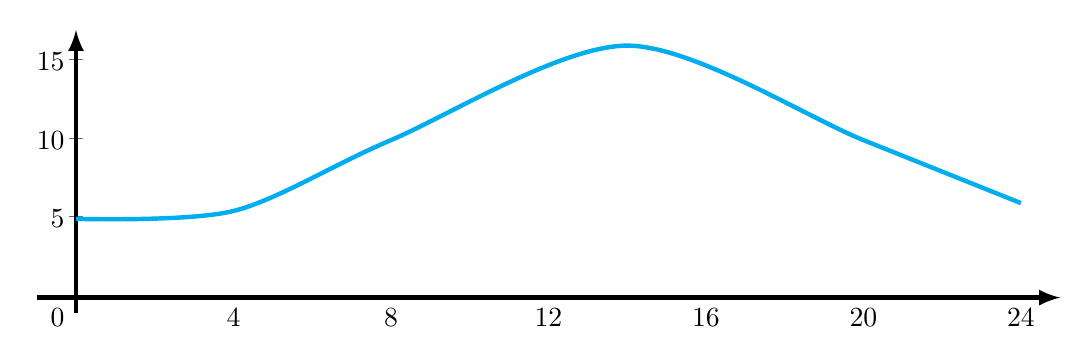
\begin{tikzpicture}[ultra thick,xscale=.5,yscale=.2]
      \draw[-latex] (-1,0) -- (25,0);
	    \draw [-latex](0,-1) -- (0, 17);
      \draw (0,0) node[below left]{0};
  \foreach \x in {4, 8, ..., 24} {
    \draw (\x, 0) node{|} node[below]{\x};
  }
  \foreach \x in {5, 10, ..., 15} {
    \draw (0, \x) node{--} node[left]{\x};
  }
	\draw [cyan] plot [smooth, tension=0.5] coordinates {
  (0,5) (4,5.5) (8,10) (14,16) (20,10) (24,6)
};
    \end{tikzpicture}
    \end{center}

  \begin{enumerate}
    \item L'ensemble de définition de $T$ est \ldots.
      \begin{multicols}{2}
    \item Les énoncés suivants sont \\équivalents.
      \begin{enumerate}
        \item L'image de 12 par $T$ est \ldots.
        \item \ldots
        \item 
      \end{enumerate}
    \item Les énoncés suivants sont \\équivalents.
      \begin{enumerate}
        \item Les antécédents de 10 par $T$ sont \ldots
        \item \ldots
        \item Il a fait 10\degre{}C à \ldots
      \end{enumerate}
    \end{multicols}
  \end{enumerate}
  \vfill

  \subsection{Volume d'un cube}
  Soit la fonction $V$ qui à une longueur $c$ associe le volume du cube de côté $c$.
  \begin{enumerate}
    \item L'expression de $V$ est \ldots
    \item Le domaine de définition de $V$ est \ldots
    \item L'image de 2 par $V$ est \ldots
    \item Le(s) antécédent(s) de 27 par  $V$ est/sont :
  \end{enumerate}

\end{document}
